This section presents the results of the proposed method applied to various datasets. The initial part of this section compares the proposed method with a related method for change point detection based on subspace identification using online SVD.~Artificial step detection highlights the significant differences in identifying subspaces using the two decomposition methods. Two real-world datasets are used to compare the performance of our proposed method with that of the alternative subspace identification method.

Secondly, we address the challenging real-world dataset involving faulty HVAC operation detection in an industrial-scale battery energy storage system (BESS). The final subsection compares the proposed method with other methods used for change-point detection on benchmarking data of a simulated complex dynamical system with control (CATS) and a laboratory water circulation system (SKAB).

\subsection{Artificial steps detection}
Change-point detection can be simplified to finding the temporal dynamics of a system not captured in data nor acknowledged by the supervisory control system. A simple artificial dataset with steps and Gaussian noise can validate the proper functioning of the proposed method. This dataset, initially proposed in~\citet{Kawahara2007}, highlights our proposed variation of online DMD as superior to online singular value decomposition.

The dataset consists of 10,000 snapshots with nine steps of increasing size and distance from the original operation point after every 1,000 snapshots. Gaussian noise is added to challenge one of the weaknesses of subspace-identification-based methods.

Our proposed method is compared to the online SVD-based CPD presented in \citet{Kawahara2007} using the same hyperparameters, as listed in Table~\ref{table:kawahara_comp_hyperparameters}.

\begin{table}[ht]
	\caption{Hyperparameters used for comparison with online SVD based CPD.}\label{table:kawahara_comp_hyperparameters}
	\centering
	\begin{tabular}{l S[table-format=3.0]}
		\toprule
		\textbf{Hyperparameter} & \textbf{Value} \\
		\midrule
		\(r\)                   & 2              \\
		\(a\)                   & 100            \\
		\(b\)                   & 0              \\
		\(c\)                   & 100            \\
		\(d\)                   & 300            \\
		\(h\)                   & 80             \\
		\bottomrule
	\end{tabular}
\end{table}

The results in Figure~\ref{fig:artificial_steps_detection} show that while no method identified the first change-point at snapshot 1000, DMD-CPD discriminates minor change-points around the first operation point, with decreasing change-point statistics for subsequent detections. This decrease can be explained by the significant increase in absolute error between the original and reconstructed data for both the base and test sets, compared to their relative error, which decreases the residual of their division. Computing the difference between test and base set reconstruction errors gives evidence to the previous explanation. This relation of energy of the change-point detection to the actual dissimilarity of the data is a significant advantage of the proposed method over the deep learning techniques~\citep{DeRyck2021}. To sum up, the absolute dissimilarity of the data is reflected in the difference in the errors, while the relative dissimilarity is reflected in the error ratio.

The proposed method has a similar shape of statistics for error divergence to the error ratio statistics of the method proposed in \citet{Kawahara2007} but with significantly lower noise. In both cases, the peak of the change-point statistics is delayed by \(c\) snapshots, which is expected due to the nature of CPD-DMD.~The exact delay allows for precisely pinpointing the change-point time.

\begin{figure}[H]
	\centering
	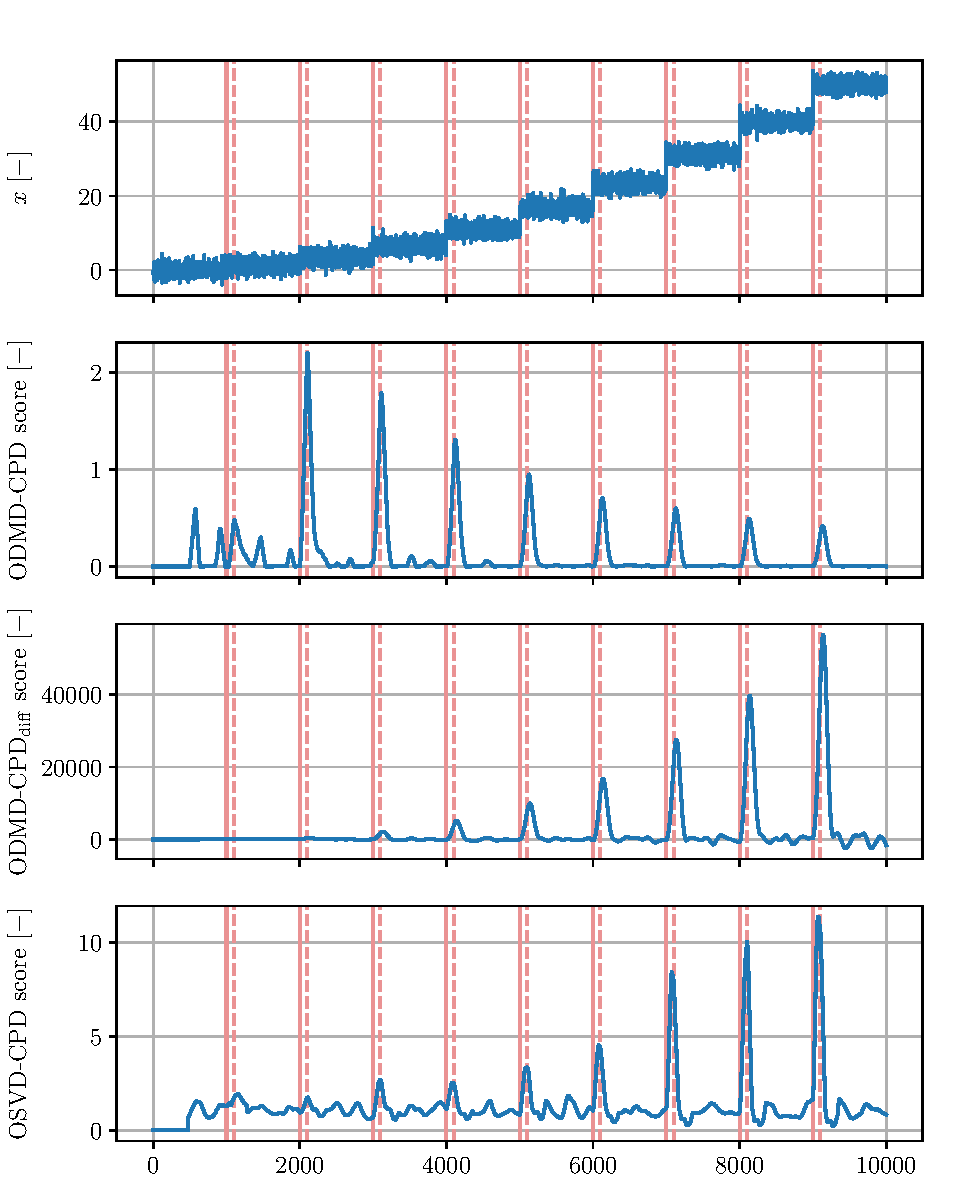
\includegraphics[width=\linewidth]{figures/y0-chd_r2_100_100-roll_301-dmd_w1.0-h80.pdf}
	\caption{Steps detection in artificial data (1). Change score is evaluated for the proposed method as presented in Section~\ref{sec:method} (2), the proposed method evaluating score as the difference of errors (3), and the reference method using online SVD (4). Our method is capable of detecting minor CPs that are missed by the reference method.}\label{fig:artificial_steps_detection}
\end{figure}

\subsection{Sleep Stage Detection via Respiration Signal}
Identifying change points in real-world data is challenging due to cyclic, seasonal, and environmental effects. In this context, we use a dataset of respiration signals from a sleep stage detection task. The datasets represent respiration (thorax extension), sampled at 10 Hz from different subjects. The data are manually labeled by Dr.~J. Rittweger from the Institute for Physiology at the Free University of Berlin. For details, refer to the original publication~\citep{Keogh2005}. For comparison with online SVD, we use the same hyperparameters as in the previous section, listed in Table~\ref{table:kawahara_comp_hyperparameters}.

\paragraph{NPRS43}
The comparison results of experiments conducted on the NPRS43 dataset are presented in Figure~\ref{fig:nprs43}. This dataset spans approximately 7 minutes of sleep respiration signals of a subject. The subject is in stage II deep sleep for the first 5 minutes, then transitions through a short awake stage of approximately 1 minute to the stage I sleep. The transitions are marked as red vertical lines in the plot. Due to the size of the test set, the peak of change-point statistics is delayed by \(c\) snapshots and marked as red dashed vertical lines.

Both methods identify the first transition from stage II to the awake state with a peak of statistics delayed by \(c\). While SVD fails to recognize the second transition, our method displays an increased score with significant delay after the transition. Since the delay is longer than \(a + c\), it could be regarded as a false positive (FP) detection of a change point. Nonetheless, by visually examining data after the ground truth label, it could be argued that the second transition occurs more gradually and spans multiple breathing cycles, two with very short thrax extensions after the ground truth label, followed by two with larger thrax extensions and ended by two very large extensions. Our method seems to capture the middle point of this gradual transition as a reference, and learning windows cross the first transition point. The validity of this reasoning was not supported by the

\begin{figure}
	\centering
	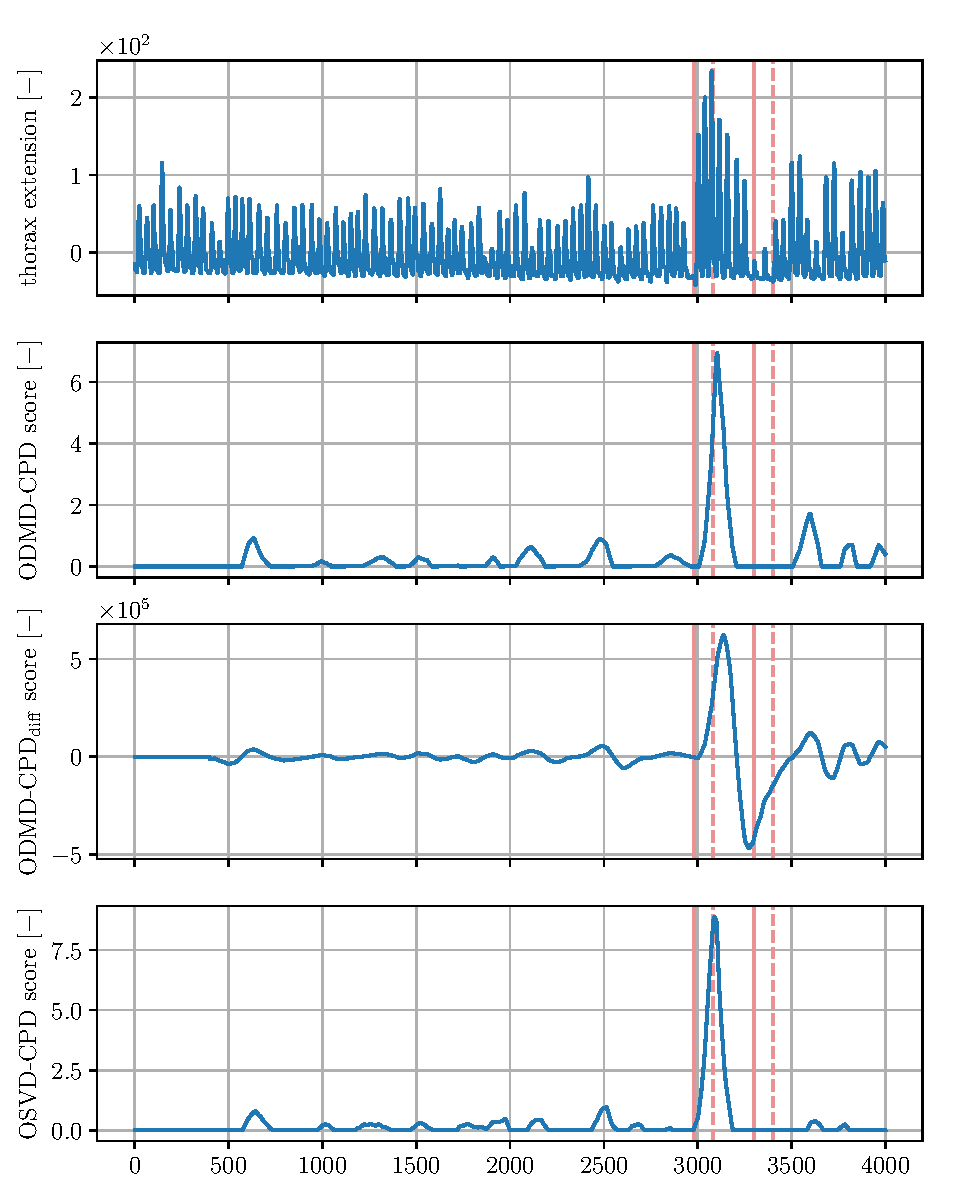
\includegraphics[width=\linewidth]{figures/nprs43-chd_r2-roll_301-dmd_w1.0-h80.pdf}
	\caption{NPRS43: Sleep stage transition detection based on respiration data (1). Change score is evaluated for the proposed method as presented in Section~\ref{sec:method} (2), the proposed method evaluating score as the difference of errors (3), and the reference method using online SVD (4). While both methods detect the first CP, our method detects the second CP as well, albeit with a longer delay due to the proximity of the CPs.}\label{fig:nprs43}
\end{figure}

\paragraph{NPRS44}
The comparison results of experiments conducted on the NPRS44 dataset are presented in Figure~\ref{fig:nprs44}. This dataset spans approximately 11 minutes of sleep respiration signals of a subject. The subject is in stage II deep sleep for the first 4 minutes, then transitions through the stage I sleep, indicated by shallow breathing, for approximately 4 minutes to an awake state. The transitions are marked as red vertical lines, and the ideal change statistics peak as grey lines in the plot.

Both methods identify the transitions present in the dataset with high discrimination capacity. CPD-DMD has significantly fewer sharp peaks in areas where a transition is not anticipated compared to the SVD-based method. Moreover, CPD-DMD captures the second transition with higher prominence and achieves peak detection with a delay of exactly \(c\) snapshots. Under the same parametrization, CPD-DMD shows smoother scores and slightly better discrimination of the transitions.

\begin{figure}[H]
	\centering
	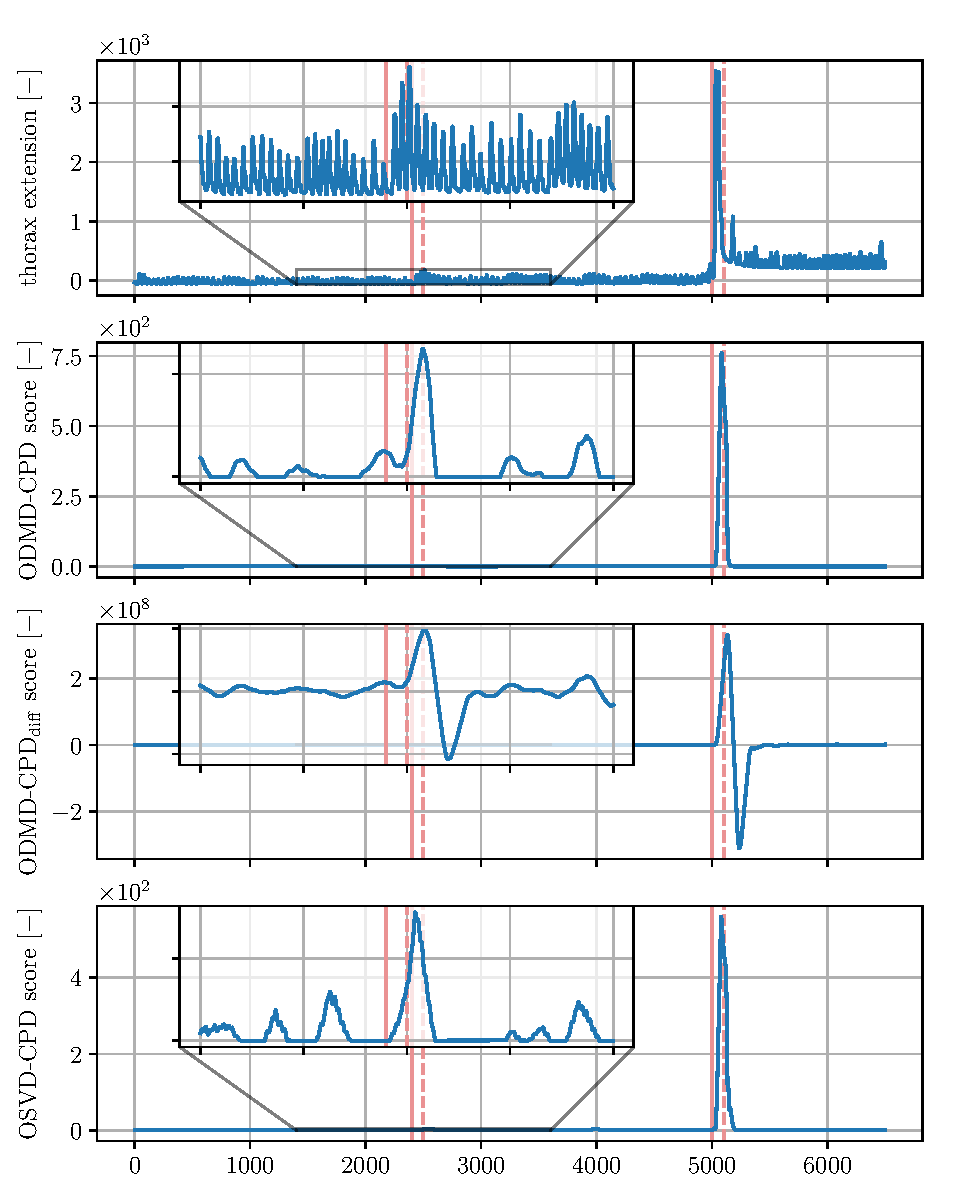
\includegraphics[width=\linewidth]{figures/nprs44-chd_r2-roll_301-dmd_w1.0-h80.pdf}
	\caption{NPRS434: Sleep stage transition detection based on respiration data (1). Change score is evaluated for the proposed method as presented in Section~\ref{sec:method} (2), the proposed method evaluating score as the difference of errors (3), and the reference method using online SVD (4). While both methods detect CPs, our method detects the first one with a score three times higher than the peaks unrelated to tracked events, while OSVD only doubles the score.}\label{fig:nprs44}
\end{figure}

\subsection{Simulated Two Tanks System with Input Delay}
To demonstrate the applicability of the proposed method to non-linear controlled systems with time delays, we demonstrate its performance on a simulated two-tank system with input delay represented by a system of ODE

\begin{equation}\label{eq:two_tanks_system}
	\begin{aligned}
		\diff{h_1(t)}{t} & = q(t-\tau) - \frac{k_1}{F_1}\sqrt{h_1(t)}                     \\
		\diff{h_2(t)}{t} & = \frac{k_1}{F_2}\sqrt{h_1(t)} - \frac{k_2}{F_2}\sqrt{h_2(t)},
	\end{aligned}
\end{equation}

where \(h_1(t)\) and \(h_2(t)\) are the levels in the tanks, \(q(t)\) is the control action, \(\tau \) is the time delay, \(k_1\) and \(k_2\) are the valve constants, and \(F_1\) and \(F_2\) are the cross-sectional areas of the tanks.

The system in Eq.~\ref{eq:two_tanks_system} is simulated with a sampling frequency of 0.1 Hz and 12,000 snapshots. After every 200 snapshots, a step change is introduced through the action of a valve selected randomly from the interval \(\interval[open left]{0.0}{0.03} m^3s^{-1}\). The time delay of the system's response to control is between 20 to 30 snapshots. The states of the system are subject to external stimuli and Gaussian noise with a variance of \(0.35\). After 4000 snapshots, the artificial sensor bias causes unit step change in the observation of tank levels for subsequent 1000 snapshots. Between 7600 and 8600, the system's response to control action is doubled, which may be caused by an offset in the control valve. Lastly, a linear trend is added to the system states between 9800 and 12000 snapshots to stimulate the increasing offset in the control.

The hyperparameters are selected based on the knowledge of the system dynamics. The learning window \(d\) is set to 2000 snapshots to capture the system's response to multiple control actions and different set points. The number of time delays in an embedding of states \(h\) is set to 200 snapshots to capture the system's dynamics, and \(\ui{h}{d}\) is set to 30 to increase performance while not significantly compromising representativeness of the dynamics. The time delays in a control action embedding are set to 30 to capture the control action responsible for the current system's response. As part of the on-the-flight preprocessing, we introduce a polynomial of degree 2 to the states to capture the non-linear dynamics of the system.~\(q\) and \(p\) are set to 2 and 1, respectively, to mitigate the impact of noise and capture information about the system's dynamics which time-delayed or polynomial embeddings might reveal.

The results of the detection experiment on the simulated data, presented in Figure~\ref{fig:non-linear}, show that the proposed method accurately detects the starts of change points in the system's operation. The peak of change-point statistics is delayed by \(c\) snapshots, which is expected due to the nature of CPD-DMD\@. The proposed method detects all the change points in the system's operation, including the artificial sensor bias, the doubled response to control action, and the linear trend in the system states. While the SVD-based method detects all the change points as well, noisy CPD statistics may hinder the recognition of another change point regarding linear trends, which may be observed more often in real scenarios due to the aging of the device and seasonal effects.

\begin{figure}[H]
	\centering
	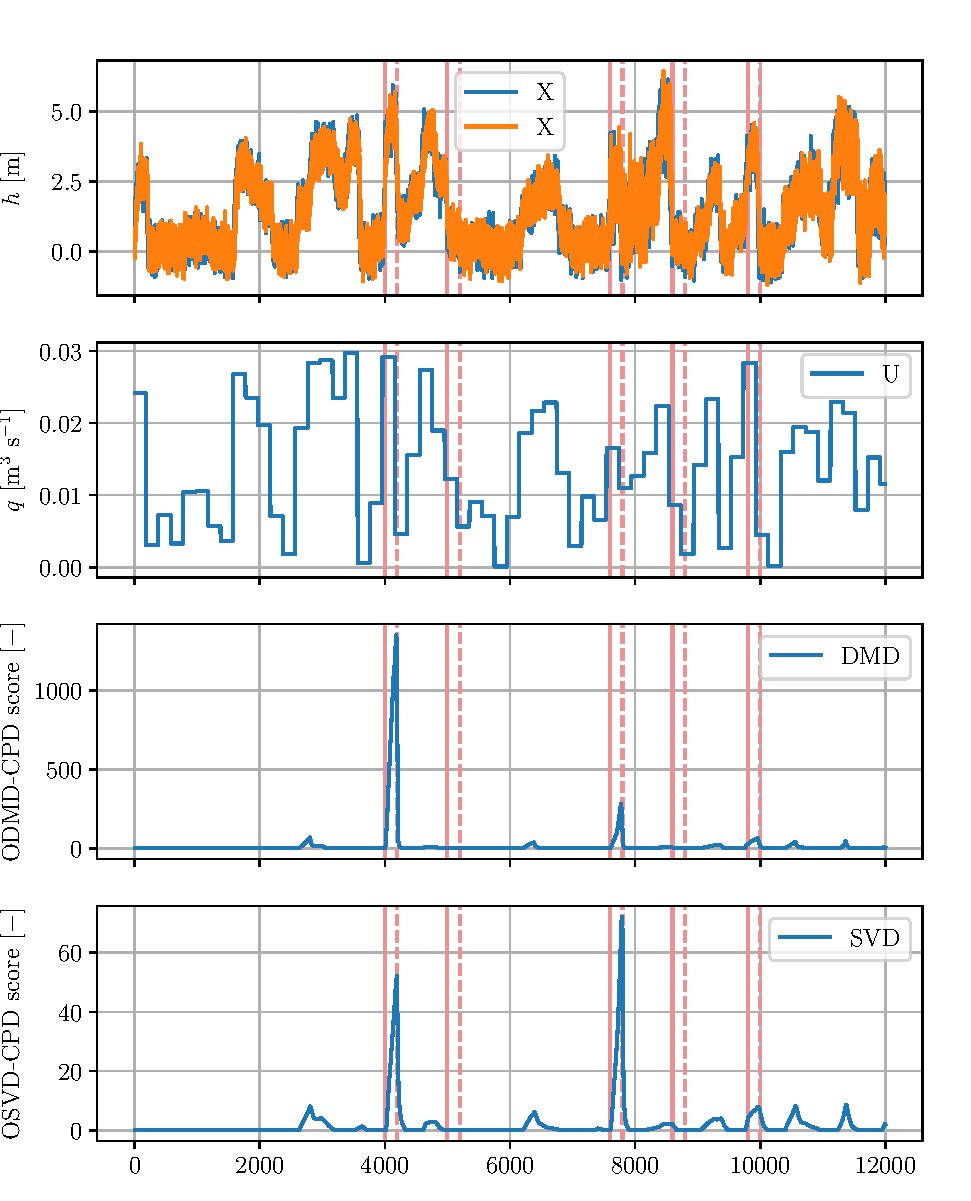
\includegraphics[width=\linewidth]{figures/nonlin-chd_p2_q1-l2000_b200_t200roll_2000-dmd_w1.0-hx15-hl30.pdf}
	\caption{CPD detection on data of two tanks system (1) with delayed input (2) shows lower noise of DMD-CPD score (3) aiding recognition of the slow drift from snapshot 9800 as compared to the reference method (4).}\label{fig:non-linear}
\end{figure}

\subsection{BESS --- Faulty HVAC Operation Detection}
This case study demonstrates detection performance on a real-world dataset of faulty HVAC operation in an industrial-scale battery energy storage system (BESS). The studied BESS has an installed capacity of 151 kWh distributed among ten modules with 20 Li-ion NMC cells. A hardware fault occurred on one of the module's cooling fans on 23rd August 2023 at 17:12:30. To protect the profitability of the BESS for the end user, the faulty BESS was operated securely until the fault was fixed. This case study aims to detect the transition from normal to faulty operation of the HVAC system based on temperature profile monitoring. The dataset is provided by the BESS operator and normalized to protect sensitive business information. It captures snapshots of six spatially distributed temperature sensors of the targeted BESS module operation at approximately 30-second intervals.

The selection of hyperparameters demonstrates the intuitiveness of parameter selection. The BESS is utilized in an industrial setting for availability time-shifting of energy generated by a solar power plant, subject to daily seasonality and weekly periodicity. The learning window \(d\) is set for 24 hours to reflect these patterns and track weekday and weekend operations well. The maximum C-rate of the BESS is 1.0, defining another important hourly time constant. With this knowledge, we can minimize the impact of charging events on change-point detection statistics; \(a\) and \(c\) window sizes are set to double the fastest charging rate, 240 samples, corresponding to 2 hours of operation. The number of time delays in the embedded matrix reflects the known dynamics of the system; hence, \(h\) is set to 240 samples.

The results of the detection experiment on simulated data streaming from the BESS history replay, presented in Figure~\ref{fig:bess}, show that before the actual occurrence of the fault, the system detects multiple events of abnormal operation with a source other than the identified dynamical system from the data. The proposed method accurately detects the transition from normal to faulty operation of the HVAC system with high accuracy and low false positive rate, with the peak of change-point statistics delayed by \(c\) snapshots.

The proposed method detected three periods related to the transient normal behavior of the HVAC system, marked as change points. While it is challenging to confirm if the initial peaks in the CPD score were false positives, operators can interpret this information as a potential early warning of an impending fault. Such early warnings are valuable for detecting faults, preventing catastrophic consequences, and planning maintenance. The positions of the potential fault precursors match the detected anomalies in~\citet{Wadinger2024}, where detection was performed using an online anomaly detection method based on conditional probability distribution. This alignment supports cross-validation of both methods and lends credibility to identifying these events as fault precursors.

The evaluation of error difference shows that we can detect both the transition from normal to faulty operation and vice versa. Here, the peaks related to true anticipated CPs are more pronounced than those in the error ratio evaluation. This indicates the usefulness of the error difference evaluation in increasing the precision of the CPD\@.

\begin{figure}[H]
	\centering
	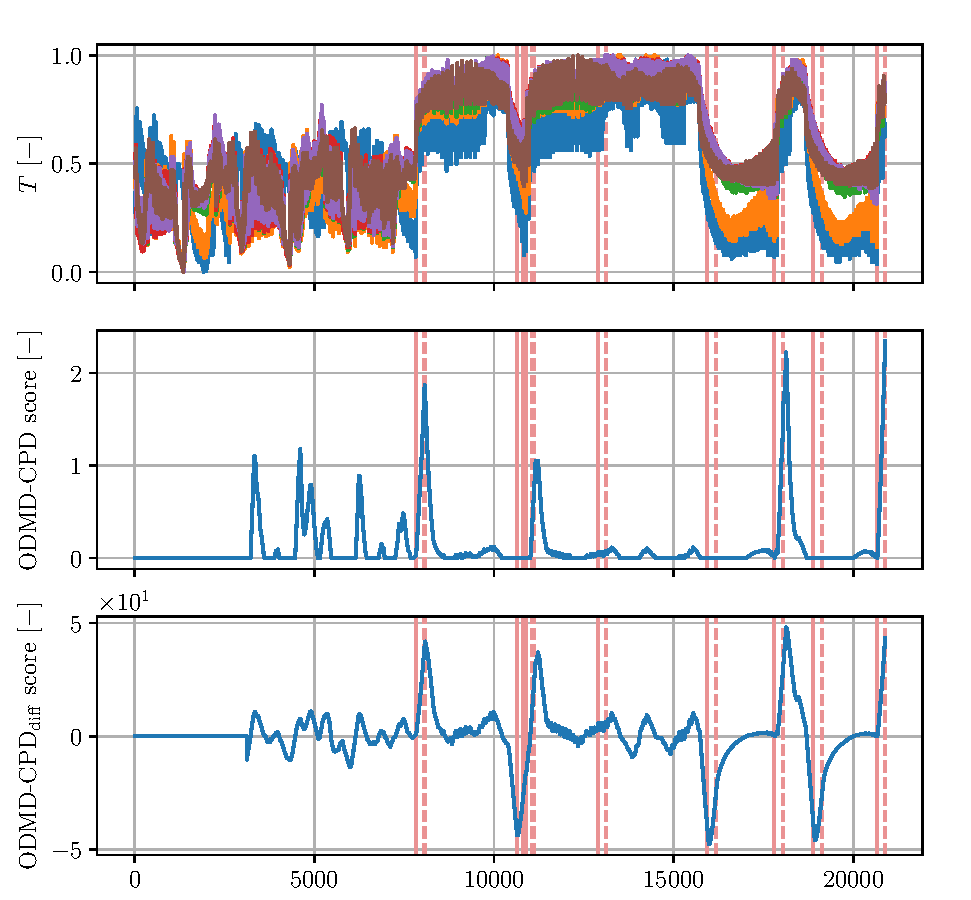
\includegraphics[width=\linewidth]{figures/bess-chd_p10-l2880_b240_t240roll_2880-dmd_w1.0-hx20.pdf}
	\caption{Faulty operation of HVAC in BESS results in altered operation temperature (1). Our proposed method detects a transition towards a novel state and displays multiple peaks in the CPD score (2). Meanwhile, an alternative formulation of our proposed method increases the prominence of the CPD score peaks during the transition towards the novel state and assigns negative peaks in the CPD score to the transitions back towards the original state (3).}\label{fig:bess}
\end{figure}

\subsection{Laboratory Water Circulation System (SKAB)}
In this section, we compare the performance of the proposed method with commonly used change-point detection methods on a benchmark real-world dataset of a laboratory water circulation system (SKAB)~\citep{Katser2020}. The dataset represents a well-described industrial system with multiple sensors and well-defined operational and fault states characterized by collective anomalies or change points, as well as transitions between these states.

\citet{Katser2020} compare methods with default hyperparameters, which are listed in Table~\ref{table:comparison-models}, using the first 400 snapshots of each dataset as a training part. We follow the same procedure, and for CPD-DMD hyperparameters with task-specific tuning requirements, we use the training set of samples as a history of snapshots to establish the parameters.

\begin{table}[H]
	\caption{List of reference method and sources}\label{table:comparison-models}
	\centering
	\begin{tabular}{l l S[table-format=3.0]}
		\toprule
		\textbf{Algorithm} & \textbf{Source}       \\
		\midrule
		Conv-AE            & \citet{Pavithra2020}  \\
		Isolation forest   & \citet{Liu2008}       \\
		LSTM-AE            & \citet{Chollet2016}   \\
		MSCRED             & \citet{ZhangCh2019}   \\
		MSET               & \citet{Gross2000}     \\
		T-squared          & \citet{Hotelling1947} \\
		T-squared+Q (PCA)  & \citet{JoeQin2003}    \\
		Vanilla AE         & \citet{Chen2017}      \\
		Vanilla LSTM       & \citet{Filonov2016}   \\
		\bottomrule
	\end{tabular}
\end{table}

The evaluation is performed using NAB metrics presented in the work of~\citet{Ahmad2017}. These metrics operate over a window of snapshots. In the leaderboard proposed in~\citet{Katser2020}, the window is centered around the change point to establish metrics for reference methods. Nevertheless, from the definition of the change-point and the utilization of the window for scoring (please refer to the paper by~\citet{Lavin2015}), it is evident that the detector alerting a change-point half of the window size snapshots before the change-point actually occurs is considered perfect. Since the start of the transition towards the faulty state is marked as anomalous in the dataset, as seen in Figure~\ref{fig:scab_interpretation}, we stipulate that the detection before the start of the transition should be regarded as a false positive. Therefore, we modify the original evaluation metrics to observe the snapshots window after the change-point and evaluate the models' performance.

To ensure reproducibility and consistency, we created a fork of the original repository available at \url{https://github.com/MarekWadinger/SKAB}.

\begin{figure}[H]
	\centering
	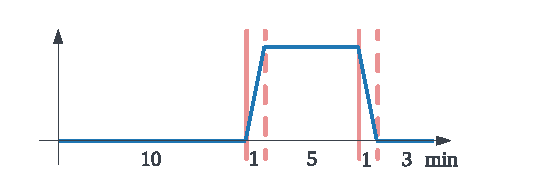
\includegraphics[width=\linewidth]{figures/scab-interpretation.pdf}
	\caption{After 10 minutes of normal behavior, the system starts transitioning to a new operating point (indicated by the solid red line), which takes 1 minute to complete (indicated by the dashed red line). The system maintains this new operating state for 5 minutes, then transitions back to the original state over the next minute.}\label{fig:scab_interpretation}
\end{figure}

The results of experiments, presented in Table~\ref{table:skab_cpd_comparison-own}, show that the proposed method outperforms the reference methods in terms of standard NAB score, low FP, and low FN scores. Our proposed method and MSCRED have the lowest number of missed change points, making them more suitable methods for safety-critical systems where missed alarms may result in catastrophic consequences. Two variants of the proposed method are evaluated to show the influence of threshold \(t\) selection. Based on the results, we claim that the selection of threshold value, which is challenging for non-probabilistic approaches to CPD where CPD statistics have no proper normalization, may improve the FP score but does not significantly impact performance. Thus, this difficult-to-select parameter can initially be set to 0 and then increased to improve the false positive score when dealing with signals that are hard to reconstruct due to significant noise. Perhaps most interesting is the score of the perfect detector, which is not 100 as expected. This indicates that the standard NAB score does not guarantee a 100 for a perfect detector for various evaluation criteria, which is essential to consider when evaluating the relative performance of the methods with respect to the perfect detector under these criteria.

\begin{table}[H]
	\caption{Comparison of different algorithms based on NAB metrics. The best scores are highlighted.}\label{table:skab_cpd_comparison-own}
	\centering
	\begin{tabular}{l *3{S[table-format=3.2]}}
		\toprule
		\textbf{Algorithm}              &
		\multicolumn{1}{p{1.7cm}}{\centering \textbf{NAB}                                  \\ (standard)} &
		\multicolumn{1}{p{1.7cm}}{\centering \textbf{NAB}                                  \\ (low FP)} &
		\multicolumn{1}{p{1.7cm}}{\centering \textbf{NAB}                                  \\ (low FN)}
		\\
		\midrule
		Perfect detector                & 54.77          & 54.11          & 56.99          \\
		\midrule
		\textbf{CPD-DMD (\(t=0\))}      & \textbf{34.29} & 23.21          & \textbf{42.54} \\
		\textbf{CPD-DMD} (\(t=0.0025\)) & 33.43          & \textbf{23.28} & 41.71          \\
		MSCRED                          & 32.42          & 16.53          & 40.28          \\
		Isolation forest                & 26.16          & 19.50          & 30.82          \\
		T-squared+Q (PCA)               & 25.35          & 14.51          & 31.33          \\
		Conv-AE                         & 23.61          & 21.54          & 27.55          \\
		LSTM-AE                         & 23.51          & 20.11          & 25.91          \\
		T-squared                       & 19.54          & 10.20          & 24.31          \\
		MSET                            & 13.84          & 10.22          & 17.37          \\
		Vanilla AE                      & 11.41          & 6.53           & 13.91          \\
		Vanilla LSTM                    & 11.31          & -3.80          & 17.25          \\
		\midrule
		% Always positive                 & 0.00           & 0.00           & 0.00           \\
		Null detector                   & 0.00           & 0.00           & 0.00           \\
		\bottomrule
	\end{tabular}
\end{table}


\subsection{Simulated Complex Dynamical System with Control (CATS)}
This section evaluates the performance of our method on the Controlled Anomalies Time Series (CATS) Dataset proposed in \citet{Fleith2023}. The dataset shows a simulation of a complex dynamical system with 200 injected anomalies, consisting of control commands, external stimuli, and 5 million snapshots of telemetry sampled at 1 Hz. While the generating mechanism is not described, the availability of the benchmark dataset, including the control action signals, makes it a good candidate for evaluating the proposed method. The dataset is meant for anomaly detection algorithms but contains numerous sequences of anomalous behavior. Compared to SKAB, this dataset has a far lower contamination level of 3.8\%, making it more suitable for evaluating the CPD performance, where events of change are underrepresented.

The evaluation uses the same metrics as the previous case study on a resampled dataset to 1-minute intervals, with a median taken for both features and targets. No public background on the generating mechanism complicated the hyperparameter selection. Based on the 58-day timespan captured in the dataset, we selected one day as the learning window and set the number of time delays to 4 hours, with a maximum limit of the final number of features set to 60. The reference window is double the size of the test window, 10 hours for the former and 5 hours for the latter. The ranks of the DMD were set to 10 and 4 for the states and control inputs, respectively.

The results of experiments, presented in Table~\ref{table:cats_cpd_comparison}, show that the proposed method outperforms all reference methods but MSCRED in terms of the standard NAB score evaluated on a 5-hour window starting to the right of the actual anomaly. While our method offers a significantly better FP score, reducing the number of false alarms, MSCRED offers a significantly better FN score. It is worth stating that while our proposed method and other reference methods completed the experiment within 1 hour, it took almost 24 hours for MSCRED\@. This means that it requires roughly one second per snapshot to process the data, which could challenge MSCRED's applicability in hard real-time scenarios with the original frequency of 1 Hz. In the given settings, our proposed method balances well between false positives and false negatives, with the lowest number of missed change points. The results indicate that the proposed method is capable of detecting change points in the complex dynamical system and can employ information about control inputs.

\begin{table}[H]
	\caption{Comparison of different algorithms based on NAB metrics. The best scores are highlighted.}\label{table:cats_cpd_comparison}
	\centering
	\begin{tabular}{l *3{S[table-format=3.2]}}
		\toprule
		\textbf{Algorithm}              &
		\multicolumn{1}{p{1.7cm}}{\centering \textbf{NAB}                                  \\ (standard)} &
		\multicolumn{1}{p{1.7cm}}{\centering \textbf{NAB}                                  \\ (low FP)} &
		\multicolumn{1}{p{1.7cm}}{\centering \textbf{NAB}                                  \\ (low FN)}
		\\
		\midrule
		Perfect detector                & 30.21          & 29.89          & 31.28          \\
		\midrule
		MSCRED                          & \textbf{37.19} & 13.46          & \textbf{47.18} \\
		\textbf{CPD-DMD (\(t=0\))}      & 25.66          & \textbf{20.62} & 29.84          \\
		\textbf{CPD-DMD}                & 17.84          & 15.01          & 20.06          \\
		Isolation forest (\(c=3.8\% \)) & 17.81          & 15.84          & 20.00          \\
		T-squared+Q (PCA)               & 11.80          & 11.40          & 12.30          \\
		LSTM-AE                         & 11.39          & 11.26          & 11.69          \\
		T-squared                       & 15.15          & 14.98          & 15.71          \\
		MSET                            & 14.48          & 13.43          & 15.60          \\
		Vanilla AE                      & 2.52           & 2.44           & 2.77           \\
		Vanilla LSTM                    & 0.73           & 0.70           & 0.82           \\
		Conv-AE                         & 0.15           & 0.14           & 0.18           \\
		\midrule
		% Always positive                & 0.00           & 0.00           & 0.00           \\
		Null detector                   & 0.00           & 0.00           & 0.00           \\
		\bottomrule
	\end{tabular}
\end{table}
